\documentclass{amsart}
\usepackage{tikz}
\usepackage{pgfplots}
\usepackage[margin=0.25in]{geometry}
\usepackage{pgfplots}
\pgfplotsset{width=12cm,compat=1.4}

\begin{document}
 
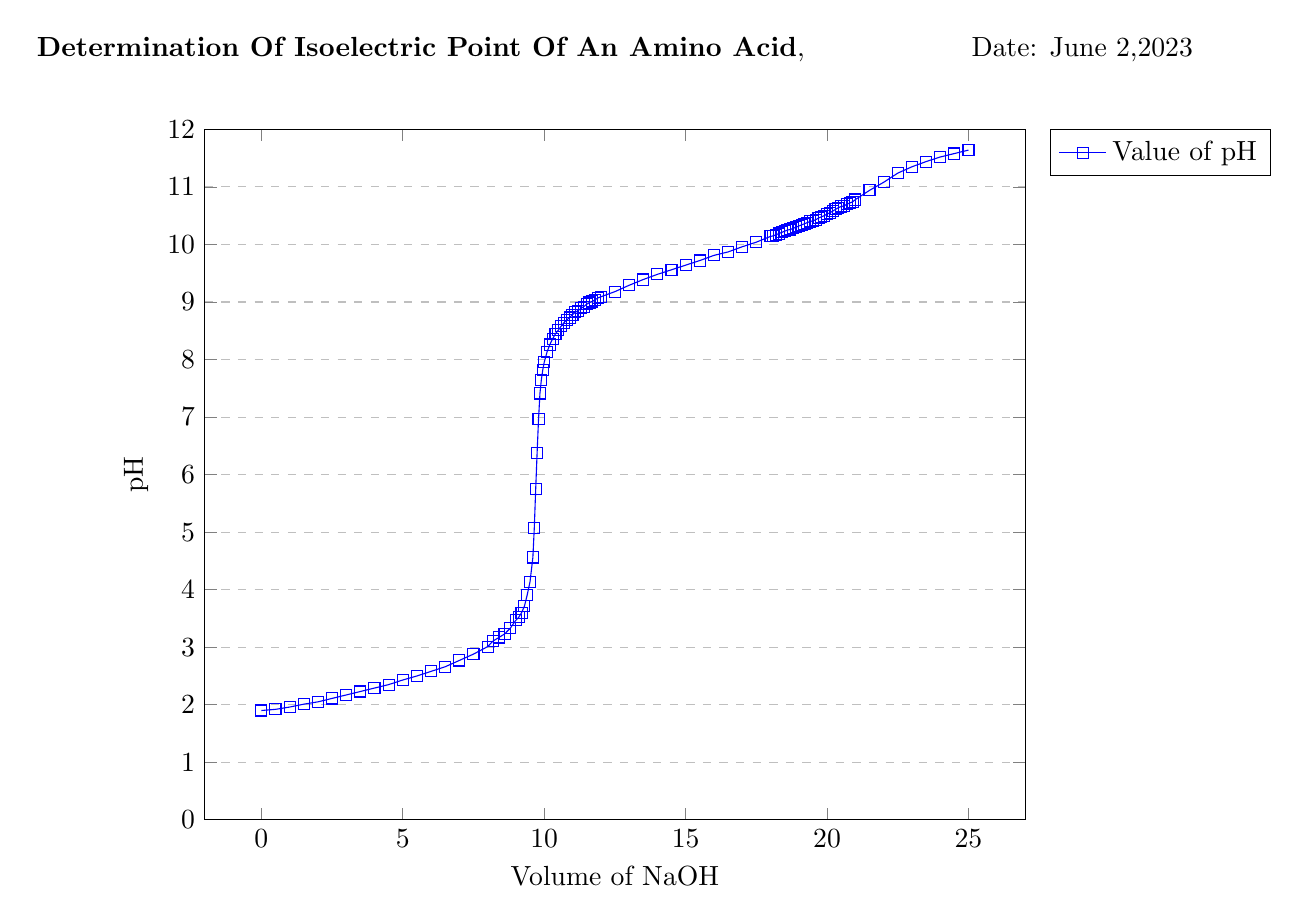
\begin{tikzpicture}
\begin{axis}[
  title={\textbf{Determination Of Isoelectric Point Of An Amino Acid},\hspace{2cm} Date: June 2,2023},
  title style={yshift=1.5em},
    xlabel={Volume of NaOH},
    ylabel={pH}, 
    xmin=-2, xmax=27,
    ymin=0, ymax=12,
    xtick={0,5,10,15,20,25},
    ytick={0,1,2,3,4,5,6,7,8,9,10,11,12},
    legend pos= outer north east,
    ymajorgrids=true,
    grid style=dashed,
    extra description={Date: June 2, 2023},
]

\addplot[
    color=blue,
    mark=square,
    ]
    coordinates {
   ( 0, 1.9 )
( 0.5, 1.92 )
( 1, 1.96 )
( 1.5, 2.01 )
( 2, 2.05 )
( 2.5, 2.11 )
( 3, 2.17 )
( 3.5, 2.23 )
( 4, 2.29 )
( 4.5, 2.35 )
( 5, 2.43 )
( 5.5, 2.5 )
( 6, 2.58 )
( 6.5, 2.66 )
( 7, 2.77 )
( 7.5, 2.88 )
( 8, 3.01 )
( 8.2, 3.11 )
( 8.4, 3.17 )
( 8.6, 3.23 )
( 8.8, 3.33 )
( 9, 3.47 )
( 9.1, 3.52 )
( 9.2, 3.6 )
( 9.3, 3.71 )
( 9.4, 3.91 )
( 9.5, 4.14 )
( 9.6, 4.56 )
( 9.65, 5.07 )
( 9.7, 5.75 )
( 9.75, 6.38 )
( 9.8, 6.96 )
( 9.85, 7.41 )
( 9.9, 7.65 )
( 9.95, 7.82 )
( 10, 7.95 )
( 10.1, 8.13 )
( 10.2, 8.26 )
( 10.3, 8.36 )
( 10.4, 8.45 )
( 10.5, 8.51 )
( 10.6, 8.58 )
( 10.7, 8.64 )
( 10.8, 8.69 )
( 10.9, 8.73 )
( 11, 8.78 )
( 11.1, 8.82 )
( 11.2, 8.85 )
( 11.3, 8.89 )
( 11.4, 8.92 )
( 11.5, 8.96 )
( 11.6, 8.99 )
( 11.7, 9.01 )
( 11.8, 9.04 )
( 11.9, 9.07 )
( 12, 9.09 )
( 12.5, 9.18 )
( 13, 9.29 )
( 13.5, 9.39 )
( 14, 9.48 )
( 14.5, 9.56 )
( 15, 9.64 )
( 15.5, 9.72 )
( 16, 9.81 )
( 16.5, 9.87 )
( 17, 9.96 )
( 17.5, 10.04 )
( 18, 10.14 )
( 18.1, 10.15 )
( 18.2, 10.17 )
( 18.3, 10.19 )
( 18.4, 10.21 )
( 18.5, 10.23 )
( 18.6, 10.25 )
( 18.7, 10.26 )
( 18.8, 10.28 )
( 18.9, 10.3 )
( 19, 10.32 )
( 19.1, 10.34 )
( 19.2, 10.36 )
( 19.3, 10.38 )
( 19.4, 10.4 )
( 19.5, 10.41 )
( 19.6, 10.43 )
( 19.7, 10.46 )
( 19.8, 10.48 )
( 19.9, 10.5 )
( 20, 10.53 )
( 20.1, 10.55 )
( 20.2, 10.58 )
( 20.3, 10.61 )
( 20.4, 10.64 )
( 20.5, 10.66 )
( 20.6, 10.67 )
( 20.7, 10.7 )
( 20.8, 10.72 )
( 20.9, 10.74 )
( 21, 10.78 )
( 21.5, 10.94 )
( 22, 11.08 )
( 22.5, 11.24 )
( 23, 11.35 )
( 23.5, 11.44 )
( 24, 11.52 )
( 24.5, 11.58 )
( 25, 11.64 )
    };
    \legend{Value of pH}
    
\end{axis}
\end{tikzpicture}


\vspace{1in}

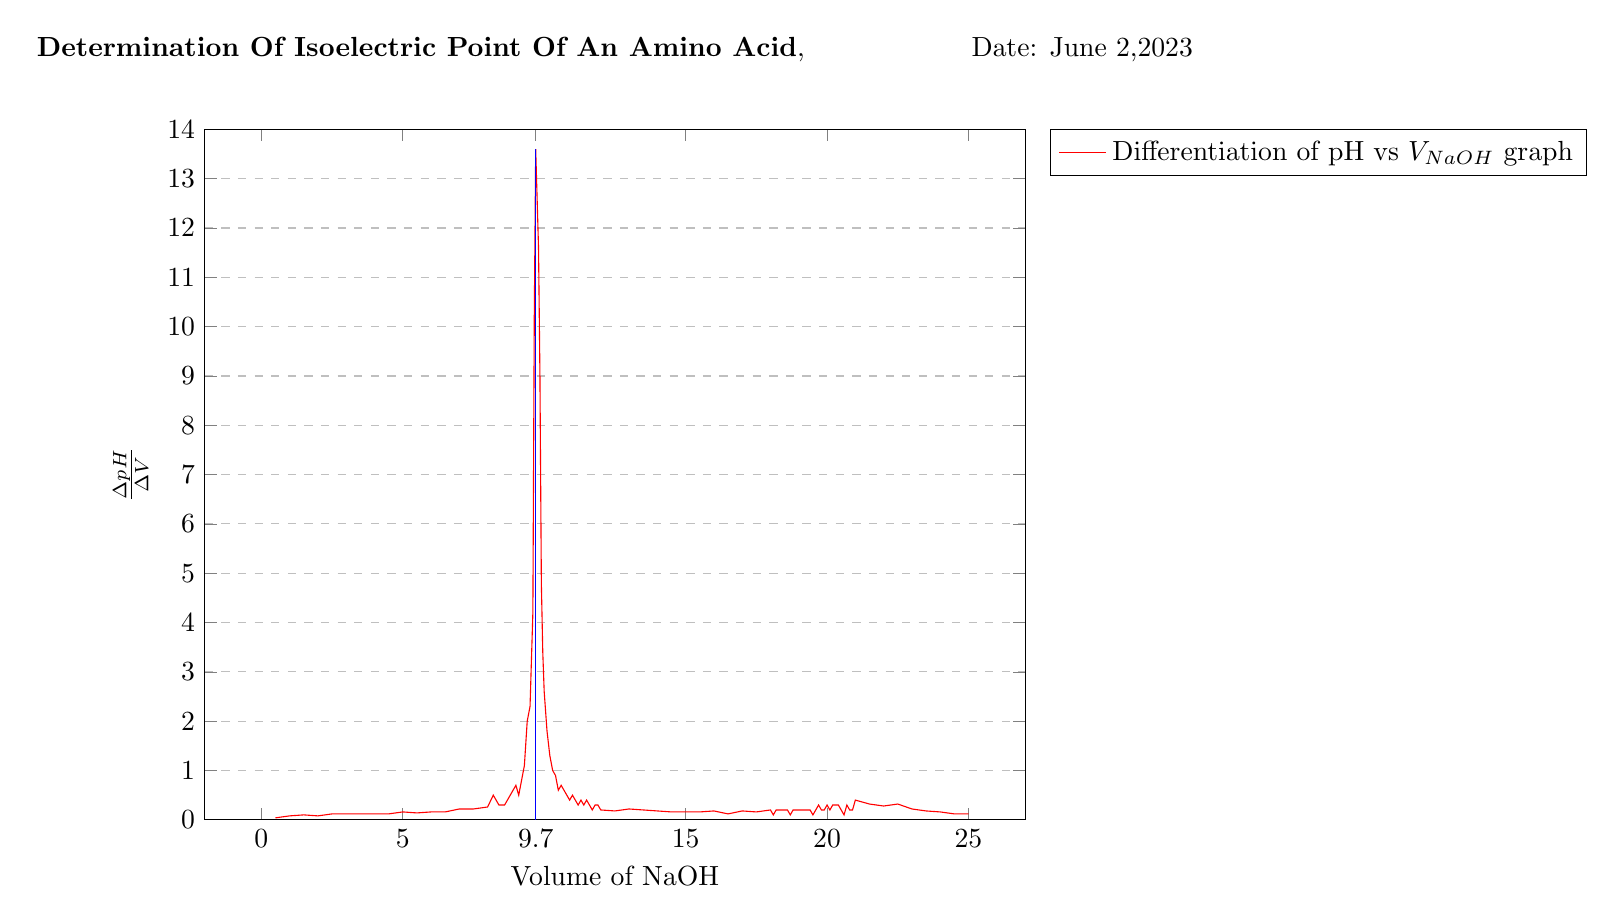
\begin{tikzpicture}
\begin{axis}[
    title={\textbf{Determination Of Isoelectric Point Of An Amino Acid},\hspace{2cm} Date: June 2,2023},
    title style={yshift=1.5em},
    xlabel={Volume of NaOH},
    ylabel={\( \frac{\Delta pH}{\Delta V}\)},
    xmin=-2, xmax=27,
    ymin=0, ymax=14,
    xtick={0,5,9.7,15,20,25},
    ytick={0,1,2,3,4,5,6,7,8,9,10,11,12,13,14},
    legend pos= outer north east,
    ymajorgrids=true,
    grid style=dashed,
    ]

\addplot[
    color=red,
    mark=circle,
    ]
    coordinates {
( 0.5, 0.04 )
( 1, 0.08 )
( 1.5, 0.1 )
( 2, 0.08 )
( 2.5, 0.12 )
( 3, 0.12 )
( 3.5, 0.12 )
( 4, 0.12 )
( 4.5, 0.12 )
( 5, 0.16 )
( 5.5, 0.14 )
( 6, 0.16 )
( 6.5, 0.16 )
( 7, 0.22 )
( 7.5, 0.22 )
( 8, 0.26 )
( 8.2, 0.5 )
( 8.4, 0.3 )
( 8.6, 0.3 )
( 8.8, 0.5 )
( 9, 0.7 )
( 9.1, 0.5 )
( 9.2, 0.8 )
( 9.3, 1.1 )
( 9.4, 2 )
( 9.5, 2.3 )
( 9.6, 4.2 )
( 9.65, 10.2 )
( 9.7, 13.6 )
( 9.75, 12.6 )
( 9.8, 11.6 )
( 9.85, 9 )
( 9.9, 4.8 )
( 9.95, 3.4 )
( 10, 2.6 )
( 10.1, 1.8 )
( 10.2, 1.3 )
( 10.3, 1 )
( 10.4, 0.9 )
( 10.5, 0.6 )
( 10.6, 0.7 )
( 10.7, 0.6 )
( 10.8, 0.5 )
( 10.9, 0.4 )
( 11, 0.5 )
( 11.1, 0.4 )
( 11.2, 0.3 )
( 11.3, 0.4 )
( 11.4, 0.3 )
( 11.5, 0.4 )
( 11.6, 0.3 )
( 11.7, 0.2 )
( 11.8, 0.3 )
( 11.9, 0.3 )
( 12, 0.2 )
( 12.5, 0.18 )
( 13, 0.22 )
( 13.5, 0.2 )
( 14, 0.18 )
( 14.5, 0.16 )
( 15, 0.16 )
( 15.5, 0.16 )
( 16, 0.18 )
( 16.5, 0.12 )
( 17, 0.18 )
( 17.5, 0.16 )
( 18, 0.2 )
( 18.1, 0.1 )
( 18.2, 0.2 )
( 18.3, 0.2 )
( 18.4, 0.2 )
( 18.5, 0.2 )
( 18.6, 0.2 )
( 18.7, 0.1 )
( 18.8, 0.2 )
( 18.9, 0.2 )
( 19, 0.2 )
( 19.1, 0.2 )
( 19.2, 0.2 )
( 19.3, 0.2 )
( 19.4, 0.2 )
( 19.5, 0.1 )
( 19.6, 0.2 )
( 19.7, 0.3 )
( 19.8, 0.2 )
( 19.9, 0.2 )
( 20, 0.3 )
( 20.1, 0.2 )
( 20.2, 0.3 )
( 20.3, 0.3 )
( 20.4, 0.3 )
( 20.5, 0.2 )
( 20.6, 0.1 )
( 20.7, 0.3 )
( 20.8, 0.2 )
( 20.9, 0.2 )
( 21, 0.4 )
( 21.5, 0.32 )
( 22, 0.28 )
( 22.5, 0.32 )
( 23, 0.22 )
( 23.5, 0.18 )
( 24, 0.16 )
( 24.5, 0.12 )
( 25, 0.12 )
};
\legend{Differentiation of pH vs \(V_{NaOH}\) graph}
\addplot[
    color=blue,
    line width=0.25pt,
    forget plot % To exclude this plot from the legend
]
    coordinates {
(9.7, 0) % Start at x=9.7 with y=0
(9.7, 13.6) % End at x=9.7 with y=14 (adjust the y-value as needed)
};
%\node at (axis cs:1, 0.5) {Author: John Doe};
\end{axis}
\end{tikzpicture}

\end{document}

